%%%%%%%%%%%%%%%%%%%%%%%%%%%%%%%%%%%%%%%%%
% Classicthesis Typographic Thesis
% LaTeX Template
% Version 1.4 (1/1/16)
%
% This template has been downloaded from:
% http://www.LaTeXTemplates.com
%
% Original author:
% André Miede (http://www.miede.de) with commenting modifications by:
% Vel (vel@LaTeXTemplates.com)
%
% License:
% GNU General Public License (v2)
%
% General Tips:
% 1) Make sure to edit the classicthesis-config.file
% 2) New enumeration (A., B., C., etc in small caps): \begin{aenumerate} \end{aenumerate}
% 3) For margin notes: \marginpar or \graffito{}
% 4) Do not use bold fonts in this style, it is designed around them
% 5) Use tables as in the examples
% 6) See classicthesis-preamble.sty for useful commands
%
%%%%%%%%%%%%%%%%%%%%%%%%%%%%%%%%%%%%%%%%%

%----------------------------------------------------------------------------------------
%	PACKAGES AND OTHER DOCUMENT CONFIGURATIONS
%----------------------------------------------------------------------------------------

\documentclass[
		twoside,openright,titlepage,numbers=noenddot,headinclude,%1headlines,
	 	footinclude=true,cleardoublepage=empty,
		dottedtoc, % Make page numbers in the table of contents flushed right with dots leading to them
		BCOR=5mm,paper=a4,fontsize=11pt, % Binding correction, paper type and font size
		english,italian, % Languages, change this to your language(s)
		]{scrreprt} 
                
% Includes the file which contains all the document configurations and packages - make sure to edit this file
%%%%%%%%%%%%%%%%%%%%%%%%%%%%%%%%%%%%%%%%%
% Classicthesis Typographic Thesis
% Configuration File
%
% This file has been downloaded from:
% http://www.LaTeXTemplates.com
%
% Original author:
% André Miede (http://www.miede.de) with extensive commenting changes by:
% Vel (vel@LaTeXTemplates.com)
%
% License:
% GNU General Public License (v2)
%
% Important note:
% The main lines to change in this file are in the DOCUMENT VARIABLES
% section, the rest of the file is for advanced configuration.
%
%%%%%%%%%%%%%%%%%%%%%%%%%%%%%%%%%%%%%%%%%

%----------------------------------------------------------------------------------------
%	CHARACTER ENCODING
%----------------------------------------------------------------------------------------

\PassOptionsToPackage{utf8}{inputenc} % Set the encoding of your files. UTF-8 is the only sensible encoding nowadays. If you can't read äöüßáéçèê∂åëæƒÏ€ then change the encoding setting in your editor, not the line below. If your editor does not support utf8 use another editor!
\usepackage{inputenc}

%----------------------------------------------------------------------------------------
%	DOCUMENT VARIABLES
%	Fill in the lines below to enter your information into the thesis template
%	Each of the commands can be cited anywhere in the thesis
%----------------------------------------------------------------------------------------

% Remove drafting to get rid of the '[ Date - classicthesis version 4.0 ]' text at the bottom of every page
\PassOptionsToPackage{eulerchapternumbers,listings,drafting, pdfspacing, subfig,beramono,eulermath,parts}{classicthesis}
% Available options: drafting parts nochapters linedheaders eulerchapternumbers beramono eulermath pdfspacing minionprospacing tocaligned dottedtoc manychapters listings floatperchapter subfig

\newcommand{\myTitle}{Calculus I\xspace}
\newcommand{\mySubtitle}{Fuck yeah\xspace}
\newcommand{\myDegree}{Magnifico\xspace}
\newcommand{\myName}{Riccardo Cereghino\xspace}
\newcommand{\myProf}{Ernesto De Vito\xspace}
\newcommand{\myOtherProf}{Put name here\xspace}
\newcommand{\mySupervisor}{Put name here\xspace}
\newcommand{\myFaculty}{Informatica\xspace}
\newcommand{\myDepartment}{DIBRIS\xspace}
\newcommand{\myUni}{Put data here\xspace}
\newcommand{\myLocation}{Rapallo\xspace}
\newcommand{\myTime}{Febbraio 2019\xspace}
\newcommand{\myVersion}{version 4.2\xspace}

%----------------------------------------------------------------------------------------
%	USEFUL COMMANDS
%----------------------------------------------------------------------------------------

\newcommand{\ie}{i.\,e.}
\newcommand{\Ie}{I.\,e.}
\newcommand{\eg}{e.\,g.}
\newcommand{\Eg}{E.\,g.} 

\newcounter{dummy} % Necessary for correct hyperlinks (to index, bib, etc.)
\providecommand{\mLyX}{L\kern-.1667em\lower.25em\hbox{Y}\kern-.125emX\@}
\newlength{\abcd} % for ab..z string length calculation

%----------------------------------------------------------------------------------------
%	PACKAGES
%----------------------------------------------------------------------------------------

\usepackage{lipsum} % Used for inserting dummy 'Lorem ipsum' text into the template

%------------------------------------------------

%\PassOptionsToPackage{ngerman,american}{babel}  % Change this to your language(s)
% Spanish languages need extra options in order to work with this template
%\PassOptionsToPackage{spanish,es-lcroman}{babel}
\usepackage{babel}

%------------------------------------------------			

\usepackage{csquotes}
\PassOptionsToPackage{%
%backend=biber, % Instead of bibtex
backend=bibtex8,bibencoding=ascii,%
language=auto,%
style=numeric-comp,%
%style=authoryear-comp, % Author 1999, 2010
%bibstyle=authoryear,dashed=false, % dashed: substitute rep. author with ---
sorting=nyt, % name, year, title
maxbibnames=10, % default: 3, et al.
%backref=true,%
natbib=true % natbib compatibility mode (\citep and \citet still work)
}{biblatex}
\usepackage{biblatex}
 
 %------------------------------------------------

\PassOptionsToPackage{fleqn}{amsmath} % Math environments and more by the AMS 
 \usepackage{amsmath}
 
 %------------------------------------------------

\PassOptionsToPackage{T1}{fontenc} % T2A for cyrillics
\usepackage{fontenc}

%------------------------------------------------

\usepackage{textcomp} % Fix warning with missing font shapes

%------------------------------------------------

\usepackage{scrhack} % Fix warnings when using KOMA with listings package  

%------------------------------------------------

\usepackage{xspace} % To get the spacing after macros right

%------------------------------------------------

\usepackage{mparhack} % To get marginpar right

%------------------------------------------------

%\usepackage{fixltx2e} % Fixes some LaTeX stuff 

%------------------------------------------------

\PassOptionsToPackage{smaller}{acronym} % Include printonlyused in the first bracket to only show acronyms used in the text
\usepackage{acronym} % Nice macros for handling all acronyms in the thesis

%\renewcommand*{\acsfont}[1]{\textssc{#1}} % For MinionPro
\renewcommand*{\aclabelfont}[1]{\acsfont{#1}}

%------------------------------------------------

\PassOptionsToPackage{pdftex}{graphicx}
\usepackage{graphicx} 

%----------------------------------------------------------------------------------------
%	FLOATS: TABLES, FIGURES AND CAPTIONS SETUP
%----------------------------------------------------------------------------------------

\usepackage{tabularx} % Better tables
\setlength{\extrarowheight}{3pt} % Increase table row height
\newcommand{\tableheadline}[1]{\multicolumn{1}{c}{\spacedlowsmallcaps{#1}}}
\newcommand{\myfloatalign}{\centering} % To be used with each float for alignment
\usepackage{caption}
\captionsetup{font=small}
\usepackage{subfig}  

%----------------------------------------------------------------------------------------
%	CODE LISTINGS SETUP
%----------------------------------------------------------------------------------------

\usepackage{listings} 
%\lstset{emph={trueIndex,root},emphstyle=\color{BlueViolet}}%\underbar} % For special keywords
\lstset{language=[LaTeX]Tex,%C++ % Specify the language(s) for listings here
morekeywords={PassOptionsToPackage,selectlanguage},
keywordstyle=\color{RoyalBlue}, % Add \bfseries for bold
basicstyle=\small\ttfamily, % Makes listings a smaller font size and a different font
%identifierstyle=\color{NavyBlue}, % Color of text inside brackets
commentstyle=\color{Green}\ttfamily, % Color of comments
stringstyle=\rmfamily, % Font type to use for strings
numbers=left, % Change left to none to remove line numbers
numberstyle=\scriptsize, % Font size of the line numbers
stepnumber=5, % Increment of line numbers
numbersep=8pt, % Distance of line numbers from code listing
showstringspaces=false, % Sets whether spaces in strings should appear underlined
breaklines=true, % Force the code to stay in the confines of the listing box
%frameround=ftff, % Uncomment for rounded frame
%frame=single, % Frame border - none/leftline/topline/bottomline/lines/single/shadowbox/L
belowcaptionskip=.75\baselineskip % Space after the "Listing #: Desciption" text and the listing box
}

%----------------------------------------------------------------------------------------
%	HYPERREFERENCES
%----------------------------------------------------------------------------------------

\PassOptionsToPackage{pdftex,hyperfootnotes=false,pdfpagelabels}{hyperref}
\usepackage{hyperref}  % backref linktocpage pagebackref
\pdfcompresslevel=9
\pdfadjustspacing=1

\hypersetup{
% Uncomment the line below to remove all links (to references, figures, tables, etc), useful for b/w printouts
%draft, 
colorlinks=true, linktocpage=true, pdfstartpage=3, pdfstartview=FitV,
% Uncomment the line below if you want to have black links (e.g. for printing black and white)
%colorlinks=false, linktocpage=false, pdfborder={0 0 0}, pdfstartpage=3, pdfstartview=FitV, 
breaklinks=true, pdfpagemode=UseNone, pageanchor=true, pdfpagemode=UseOutlines,%
plainpages=false, bookmarksnumbered, bookmarksopen=true, bookmarksopenlevel=1,%
hypertexnames=true, pdfhighlight=/O,%nesting=true,%frenchlinks,%
urlcolor=webbrown, linkcolor=RoyalBlue, citecolor=webgreen, %pagecolor=RoyalBlue,%
    %urlcolor=Black, linkcolor=Black, citecolor=Black, %pagecolor=Black,%
%------------------------------------------------
% PDF file meta-information
pdftitle={\myTitle},
pdfauthor={\textcopyright\ \myName, \myUni, \myFaculty},
pdfsubject={},
pdfkeywords={},
pdfcreator={pdfLaTeX},
pdfproducer={LaTeX with hyperref and classicthesis}
%------------------------------------------------
}

%----------------------------------------------------------------------------------------
%	AUTOREFERENCES SETUP
%	Redefines how references in text are prefaced for different 
%	languages (e.g. "Section 1.2" or "section 1.2")
%----------------------------------------------------------------------------------------

\makeatletter
\@ifpackageloaded{babel}
{
\addto\extrasamerican{
\renewcommand*{\figureautorefname}{Figure}
\renewcommand*{\tableautorefname}{Table}
\renewcommand*{\partautorefname}{Part}
\renewcommand*{\chapterautorefname}{Chapter}
\renewcommand*{\sectionautorefname}{Section}
\renewcommand*{\subsectionautorefname}{Section}
\renewcommand*{\subsubsectionautorefname}{Section}
}
\addto\extrasngerman{
\renewcommand*{\paragraphautorefname}{Absatz}
\renewcommand*{\subparagraphautorefname}{Unterabsatz}
\renewcommand*{\footnoteautorefname}{Fu\"snote}
\renewcommand*{\FancyVerbLineautorefname}{Zeile}
\renewcommand*{\theoremautorefname}{Theorem}
\renewcommand*{\appendixautorefname}{Anhang}
\renewcommand*{\equationautorefname}{Gleichung}
\renewcommand*{\itemautorefname}{Punkt}
}
\providecommand{\subfigureautorefname}{\figureautorefname} % Fix to getting autorefs for subfigures right
}{\relax}
\makeatother

\usepackage{amssymb}

\let\numberset\mathbb
\newcommand{\N}{\numberset{N}}
\newcommand{\Z}{\numberset{Z}}
\newcommand{\Q}{\numberset{Q}}
\newcommand{\R}{\numberset{R}}
\newcommand{\C}{\numberset{C}}
\newcommand{\U}{\numberset{U}}
\newcommand{\I}{\numberset{I}}
\newcommand{\PP}{\numberset{P}}
\newcommand{\CC}{\complement}
\newcommand{\dom}{\text{dom }}
\newcommand{\im}{\text{Im }}
\usepackage{float}
\usepackage{wrapfig}
%----------------------------------------------------------------------------------------

\usepackage{classicthesis} 

%----------------------------------------------------------------------------------------
%	CHANGING TEXT AREA 
%----------------------------------------------------------------------------------------

%\linespread{1.05} % a bit more for Palatino
%\areaset[current]{312pt}{761pt} % 686 (factor 2.2) + 33 head + 42 head \the\footskip
%\setlength{\marginparwidth}{7em}%
%\setlength{\marginparsep}{2em}%

%----------------------------------------------------------------------------------------
%	USING DIFFERENT FONTS
%----------------------------------------------------------------------------------------

%\usepackage[oldstylenums]{kpfonts} % oldstyle notextcomp
%\usepackage[osf]{libertine}
%\usepackage[light,condensed,math]{iwona}
%\renewcommand{\sfdefault}{iwona}
%\usepackage{lmodern} % <-- no osf support :-(
%\usepackage{cfr-lm} % 
%\usepackage[urw-garamond]{mathdesign} <-- no osf support :-(
%\usepackage[default,osfigures]{opensans} % scale=0.95 
%\usepackage[sfdefault]{FiraSans}


%\addbibresource{Bibliography.bib} % The file housing your bibliography
%\addbibresource[label=ownpubs]{Self_Publications.bib} % Uncomment for optional self-publications

%\hyphenation{Put special hyphenation here}

\begin{document}

\frenchspacing % Reduces space after periods to make text more compact

\raggedbottom % Makes all pages the height of the text on that page

\selectlanguage{italian} % Select your default language - e.g. american or ngerman

%\renewcommand*{\bibname}{new name} % Uncomment to change the name of the bibliography
%\setbibpreamble{} % Uncomment to include a preamble to the bibliography - some text before the reference list starts

\pagenumbering{roman} % Roman page numbering prior to the start of the thesis content (i, ii, iii, etc)

\pagestyle{plain} % Suppress headers for the pre-content pages

%----------------------------------------------------------------------------------------
%	PRE-CONTENT THESIS PAGES
%----------------------------------------------------------------------------------------

% Title Page

\begin{titlepage}

\begin{addmargin}[-1cm]{-3cm}
\begin{center}
\large

\hfill
\vfill

\begingroup
\color{Maroon}\spacedallcaps{\myTitle} \\ \bigskip % Thesis title
\endgroup

\spacedlowsmallcaps{\myName} % Your name

\vfill


\includegraphics[width=6cm]{gfx/TFZsuperellipse_bw} \\ \medskip % Picture

\mySubtitle \\ \medskip % Thesis subtitle
%\myDegree \\
%\myDepartment \\
%\myFaculty \\
%\myUni \\ \bigskip

\myTime\ -- \myVersion % Time and version

\vfill

\end{center}
\end{addmargin}

\end{titlepage} % Main title page

\thispagestyle{empty}

\hfill

\vfill

\noindent\myName: \textit{\myTitle,} \mySubtitle, %\myDegree,
\textcopyright\ \myTime

%\bigskip
%
%\noindent\spacedlowsmallcaps{Supervisors}: \\
%\myProf \\
%\myOtherProf \\
%\mySupervisor
%
%\medskip
%
%\noindent\spacedlowsmallcaps{Location}: \\
%\myLocation
%
%\medskip
%
%\noindent\spacedlowsmallcaps{Time Frame}: \\
%\myTime
 % Back of the title page

\cleardoublepage% Dedication

\thispagestyle{empty}
\refstepcounter{dummy}

\pdfbookmark[1]{Dediche}{Dediche} % Bookmark name visible in a PDF viewer

\vspace*{3cm}

\begin{center}
\emph{Batman} Grazie di esistere    
\end{center}

\medskip

\begin{center}
Di nuovo grazie
\end{center} % Dedication page

%\cleardoublepage\include{FrontBackMatter/Foreword} % Uncomment and create a Foreword.tex to include a foreword

\cleardoublepage%*******************************************************
% Abstract
%*******************************************************
%\renewcommand{\abstractname}{Abstract}
\pdfbookmark[1]{Abstract}{Abstract}
% \addcontentsline{toc}{chapter}{\tocEntry{Abstract}}
\begingroup
\let\clearpage\relax
\let\cleardoublepage\relax
\let\cleardoublepage\relax

\chapter*{Abstract}
Short summary of the contents in English\dots a great guide by
Kent Beck how to write good abstracts can be found here:
\begin{center}
\url{https://plg.uwaterloo.ca/~migod/research/beckOOPSLA.html}
\end{center}

\vfill

\begin{otherlanguage}{ngerman}
\pdfbookmark[1]{Zusammenfassung}{Zusammenfassung}
\chapter*{Zusammenfassung}
Kurze Zusammenfassung des Inhaltes in deutscher Sprache\dots
\end{otherlanguage}

\endgroup

\vfill
 % Abstract page

%\cleardoublepage% Publications - a page listing research articles written using content in the thesis

\pdfbookmark[1]{Publications}{Publications} % Bookmark name visible in a PDF viewer

\chapter*{Publications} % Publications page text

Some ideas and figures have appeared previously in the following publications:\\

\noindent Put your publications from the thesis here. The packages \texttt{multibib} or \texttt{bibtopic} etc. can be used to handle multiple different bibliographies in your document.

%\begin{refsection}[ownpubs]
%    \small
%    \nocite{*} % is local to to the enclosing refsection
%    \printbibliography[heading=none]
%\end{refsection}

%\emph{Attention}: This requires a separate run of \texttt{bibtex} for your \texttt{refsection}, \eg, \texttt{ClassicThesis1-blx} for this file. You might also use \texttt{biber} as the backend for \texttt{biblatex}. See also \url{http://tex.stackexchange.com/questions/128196/problem-with-refsection}. % Publications from the thesis page

%\cleardoublepage% Acknowledgements

\pdfbookmark[1]{Acknowledgements}{Acknowledgements} % Bookmark name visible in a PDF viewer

\begin{flushright}{\slshape    
We have seen that computer programming is an art, \\ 
because it applies accumulated knowledge to the world, \\ 
because it requires skill and ingenuity, and especially \\
because it produces objects of beauty.} \\ \medskip
--- \defcitealias{knuth:1974}{Donald E. Knuth}\citetalias{knuth:1974} \citep{knuth:1974}
\end{flushright}

\bigskip

%----------------------------------------------------------------------------------------

\begingroup

\let\clearpage\relax
\let\cleardoublepage\relax
\let\cleardoublepage\relax

\chapter*{Acknowledgements}

\noindent Put your acknowledgements here.\\

\noindent Many thanks to everybody who already sent me a postcard!\\

\noindent Regarding the typography and other help, many thanks go to Marco Kuhlmann, Philipp Lehman, Lothar Schlesier, Jim Young, Lorenzo Pantieri and Enrico Gregorio\footnote{Members of GuIT (Gruppo Italiano Utilizzatori di \TeX\ e \LaTeX )}, J\"org Sommer, Joachim K\"ostler, Daniel Gottschlag, Denis Aydin, Paride Legovini, Steffen Prochnow, Nicolas Repp, Hinrich Harms, Roland Winkler, and the whole \LaTeX-community for support, ideas and some great software.

\bigskip

\noindent\emph{Regarding \mLyX}: The \mLyX\ port was initially done by
\emph{Nicholas Mariette} in March 2009 and continued by
\emph{Ivo Pletikosi\'c} in 2011. Thank you very much for your work and the contributions to the original style.

\endgroup % Acknowledgements page

\pagestyle{scrheadings} % Show chapter titles as headings

\cleardoublepage% Table of Contents - List of Tables/Figures/Listings and Acronyms

\refstepcounter{dummy}

\pdfbookmark[1]{\contentsname}{tableofcontents} % Bookmark name visible in a PDF viewer

\setcounter{tocdepth}{2} % Depth of sections to include in the table of contents - currently up to subsections

\setcounter{secnumdepth}{3} % Depth of sections to number in the text itself - currently up to subsubsections

\manualmark
\markboth{\spacedlowsmallcaps{\contentsname}}{\spacedlowsmallcaps{\contentsname}}
\tableofcontents 
\automark[section]{chapter}
\renewcommand{\chaptermark}[1]{\markboth{\spacedlowsmallcaps{#1}}{\spacedlowsmallcaps{#1}}}
\renewcommand{\sectionmark}[1]{\markright{\thesection\enspace\spacedlowsmallcaps{#1}}}

\clearpage

\begingroup 
\let\clearpage\relax
\let\cleardoublepage\relax
\let\cleardoublepage\relax

%----------------------------------------------------------------------------------------
%	List of Figures
%----------------------------------------------------------------------------------------

\refstepcounter{dummy}
%\addcontentsline{toc}{chapter}{\listfigurename} % Uncomment if you would like the list of figures to appear in the table of contents
\pdfbookmark[1]{\listfigurename}{lof} % Bookmark name visible in a PDF viewer

\listoffigures

\vspace{8ex}
\newpage

%----------------------------------------------------------------------------------------
%	List of Tables
%----------------------------------------------------------------------------------------

\refstepcounter{dummy}
%\addcontentsline{toc}{chapter}{\listtablename} % Uncomment if you would like the list of tables to appear in the table of contents
\pdfbookmark[1]{\listtablename}{lot} % Bookmark name visible in a PDF viewer

\listoftables
        
\vspace{8ex}
\newpage
    
%----------------------------------------------------------------------------------------
%	List of Listings
%---------------------------------------------------------------------------------------- 

\refstepcounter{dummy}
%\addcontentsline{toc}{chapter}{\lstlistlistingname} % Uncomment if you would like the list of listings to appear in the table of contents
\pdfbookmark[1]{\lstlistlistingname}{lol} % Bookmark name visible in a PDF viewer

\lstlistoflistings 

\vspace{8ex}
\newpage
       
%----------------------------------------------------------------------------------------
%	Acronyms
%----------------------------------------------------------------------------------------

\refstepcounter{dummy}
%\addcontentsline{toc}{chapter}{Acronyms} % Uncomment if you would like the acronyms to appear in the table of contents
\pdfbookmark[1]{Acronyms}{acronyms} % Bookmark name visible in a PDF viewer

\markboth{\spacedlowsmallcaps{Acronyms}}{\spacedlowsmallcaps{Acronyms}}

\chapter*{Acronyms}

\begin{acronym}[UML]
\acro{DRY}{Don't Repeat Yourself}
\acro{API}{Application Programming Interface}
\acro{UML}{Unified Modeling Language}
\end{acronym}  
                   
\endgroup % Contents, list of figures/tables/listings and acronyms

\cleardoublepage

\pagenumbering{arabic} % Arabic page numbering for thesis content (1, 2, 3, etc)
%\setcounter{page}{90} % Uncomment to manually start the page counter at an arbitrary value (for example if you wish to count the pre-content pages in the page count)

\cleardoublepage % Avoids problems with pdfbookmark

%----------------------------------------------------------------------------------------
%	THESIS CONTENT - CHAPTERS
%----------------------------------------------------------------------------------------

%\ctparttext{You can put some informational part preamble text here. Illo principalmente su nos. Non message \emph{occidental} angloromanic da. Debitas effortio simplificate sia se, auxiliar summarios da que, se avantiate publicationes via. Pan in terra summarios, capital interlingua se que. Al via multo esser specimen, campo responder que da. Le usate medical addresses pro, europa origine sanctificate nos se.} % Text on the Part 1 page describing  the content in Part 1
\ctparttext{Argomenti introduttivi del corso}
\part{Introduzione} % First part of the thesis

% Chapter 1

\chapter{Notazione} % Chapter title

\label{ch:notazione} % For referencing the chapter elsewhere, use \autoref{ch:introduction} 

%----------------------------------------------------------------------------------------
Un richiamo alla notazione che verrà utilizzata nel documento.

\section{Insiemistica}
\begin{tabular}{|l|l|}
  \hline
  $\emptyset$ & Insieme vuoto \\
  $\N$ & Insieme dei numeri naturali compreso lo $0$ \\
  $\Z$ & Insieme dei numeri relativi \\
  $\Q$ & Insieme dei numeri razionali \\
  $\R$ & Insieme dei numeri reali \\\hline
\end{tabular}

\section{Simboli logici}
\begin{tabular}{|l|l|}
  \hline
  $| $ & tale che \\
  $ \Rightarrow $ & implica \\
  $ \Leftrightarrow $ & se e solo se \\
  $ \forall $ & per ogni \\
  $ \exists $ & esiste \\
  $ \nexists $ & non esiste \\
  $ \in $ & appartiene \\
  $ \notin $ & non appartiene \\\hline
\end{tabular}



\subsection{Intervalli}
\begin{tabular}{|l|l|}
\hline
intervallo limitato chiuso &$[a,b] = \left\{ x\in \R \middle| a \leq x \leq b \right\}$ \\
intervallo limitato aperto&$(a,b) = \left\{ x\in \R \middle| a < x < b \right\}$ \\
intervallo limitato aperto a destra&$[a,b) = \left\{ x\in \R \middle| a \leq x < b \right\}$ \\
intervallo limitato aperto a sinistra&$(a,b] = \left\{ x\in \R \middle| a < x \leq b \right\}$ \\
intervallo illimitato chiuso a sinistra&$[a,+\infty) = \left\{ x\in \R \middle| x \geq a \right\}$ \\
intervallo illimitato aperto a sinistra&$(a,+\infty) = \left\{ x\in \R \middle| x > a \right\}$ \\
intervallo illimitato chiuso a destra&$(-\infty,b] = \left\{ x\in \R \middle| x \leq b \right\}$ \\
intervallo illimitato aperto a destra&$(-\infty,b) = \left\{ x\in \R \middle| x < b \right\}$ \\
intervallo illimitato&$(-\infty,+\infty) = \R$ \\ \hline
\end{tabular}

\section{Insiemi}
\subsection{Relazioni tra insiemi}
Dati due insiemi $A$ e $B$:

\begin{description}
  \item[Inclusione:] si dice che $A$ è un sottoinsieme di $B$, o che è contenuto in $B$:
    \[A \subseteq  B\]
    \[\forall x \in A \Rightarrow x \in B\]
  \item[Inclusione propria:]
    \[A \subsetneqq  B\]
    \[
      \begin{cases}
        \forall x \in A \Rightarrow x \in B \\
        \exists x \in B | x \notin A
        \end{cases}
      \]
\end{description}

\subsection{Operazioni tra insiemi}
\begin{description}
  \item[Intersezione:]
    \[A \cap B = \left\{ x \in X \middle| x \in A, x \in B\right\}\]
  \item[Unione:]
    \[A \cup B = \left\{ x \in X \middle| x \in A or x \in B\right\}\]
  \item[Differenza insiemistica:]
    \[A \diagdown B = \left\{ x \in X \middle| x \in A, x \notin B\right\}\]
  \item[Complementare:]
    \[A^C = \left\{ x \in X \middle| x \notin A \right\}\]
  \item[Prodotto cartesiano:] dove $(x,y)$ denota la coppia ordinata
  \[A\times B = \left\{ (x,y) \middle| x\in A, y\in B\right\}\]
\end{description}

\section{Numeri reali}
Dati $x,y,z \in \R$ sono definite le operazioni di:
\begin{itemize}
\item somma $x+y$
\item prodotto $xy$
\item relazione d'ordine $x<y$
\end{itemize}
Che soddisfano le seguenti proprietà:

\begin{description}
  \item[Associativa.]
    \[(x+y)+z=x+(y+z)=x+y+z \]
    \[(xy)z=x(yz)=xyz \]
  \item[Commutativa.]
    \[x+y=y+x\]
    \[xy=yx\]
  \item[Distributiva.]
    \[x(y+z)=xy+xz\]
  \item[Esistenza dell'elemento neutro.]
    \[x+0=0+x=x\]
    \[1x=x1=x\]
  \item[Esistenza dell'inverso.]
      \[\forall x \in \R \quad \exists !x=-x \in \R | x+(-x)=0\]
      \[\forall x \in \R \quad x \neq 0 \quad \exists !y=\frac{1}{x} \in \R | x\frac{1}{x}=1 \]
  \item[Relazione d'ordine totale.] per ogni $x,y,z \in \R$ una ed una sola delle seguenti relazioni è vera.
    \[
    \begin{cases}
      x<y \\
      x=y \\
      x>y
    \end{cases}
    \]
  \item[Transitiva.]
    \[(x<y) \cap (y<z) \Rightarrow (x<z)\]
  \item[Compatibilità con la somma.]
    \[x<y \Rightarrow x+z<y+z\]
  \item[Compatibilità con il prodotto.]
    \[x<y \cap z>0 \Rightarrow xz<yz\]
    \[x<y \cap z<0 \Rightarrow xz>yz\]
\end{description}

\section{Geometria}
\subsection{Circonferenza}
Dato il centro di una circonferenza $C=(x_c,y_c)$
Si esprime l'equazione della circonferenza nella forma:
\[(x-x_c)^2+(y-y_c)^2=r^2\]
Oppure:
\[x^2+y^2+\alpha x+ \beta y +\gamma =r^2\]
Per cui se $O=(0,0)$
\[x^2+y^2=r^2\]


\subsubsection{Forma canonica:}
\[\alpha = -2x_c \quad \beta = -2y_c \quad \gamma = x_c^2 + y_c^2 - r^2\]
\[x^2+y^2+\alpha x+ \beta y +\gamma =r^2\]

Per ricavare il centro:
\[C=\left(-\frac{\alpha}{2}, -\frac{\beta}{2}\right)\]
Per ricavare il raggio:
\[r=\sqrt{\frac{\alpha^2}{4}+\frac{\beta^2}{4}-\gamma}\]

\section{Ellisse}
Equazione dell'ellisse (con centro nell'origine degli assi)
\[\frac{x^2}{a^2}+\frac{y^2}{b^2} \qquad a\neq 0 , b\neq 0\]
 % Chapter 1

\cleardoublepage % Empty page before the start of the next part

%------------------------------------------------

%\ctparttext{You can put some informational part preamble text here. Illo principalmente su nos. Non message \emph{occidental} angloromanic da. Debitas effortio simplificate sia se, auxiliar summarios da que, se avantiate publicationes via. Pan in terra summarios, capital interlingua se que. Al via multo esser specimen, campo responder que da. Le usate medical addresses pro, europa origine sanctificate nos se.} % Text on the Part 2 page describing the content in Part 2

\part{Funzioni} % Second part of the thesis

% Chapter 2

\chapter{Funzioni elementari di variabile reale} % Chapter title

\label{ch:funzioni-elementari} % For referencing the chapter elsewhere, use \autoref{ch:introduction} 

%----------------------------------------------------------------------------------------

\section{Il concetto di funzione}
\textbf{Definizione:} una funzione $f: A \rightarrow \R$ dove $A \subseteq \R$ è una legge che assegna ad ogni $x\in A$ uno ed un solo valore $y=f(x) \in \R$

\textit{Nota:} in questo caso, i valori di $A$ sono chiamati variabile indipendente $(x)$, mentre  $\R$ è la variabile dipendente $y=f(x)$

\textit{Nota:} inoltre definiamo $A=dom \quad f$ come il dominio della funzione.

\textbf{Definizione:} Il grafico di $f$:
	\[f=\left\{ (x,y) \in \R^2 \middle| x \in A, y=f(x) \right\}\]

\textbf{Definizione:} L'immagine di $f$, Im f:
	\[f(A)=\left\{ f(x) \in \R \middle| x \in A \right\}\]

\section{Operazioni tra funzioni}
Date due funzioni $f:A\rightarrow \R \qquad g:B\rightarrow \R$
\begin{description}
	\item[Somma e differenza:] $(f+g)(x)=f(x)+g(x) \qquad dom(f+g)=A\cap B$
	\item[Prodotto:] $(fg)(x)=f(x)g(x) \quad dom(fg)=(A\cap B)$
	\item[Rapporto:] $(\frac{f}{g})(x)=f(x)g(x) \quad dom(\frac{f}{g})=\{x\in \R | x\in A, x\in B, g(x) \neq 0\}$
	\item[Reciproco:] $\frac{1}{f}(x)=\frac{1}{f(x)}=[f(x)]^{-1} \quad dom(\frac{1}{f})={x\in A | f(x) \neq 0}$
\end{description}

\subsection{Nomenclatura}
Data una funzione $f: A \rightarrow \R , \quad y=f(x)$
\begin{itemize}
	\item $f$ è detta \textbf{iniettiva} se $\forall y_0 \in \R , f(x)=y_0$ ha al più una soluzione.
	\item $f$ è detta \textbf{surgettiva} se $\forall y_0 \in \R , f(x)=y_0$ ha almeno una soluzione.
	\item $f$ è detta \textbf{bigettiva} se $\forall y_0 \in \R , f(x)=y_0$ ha una ed una sola soluzione, ovvero se la funzione è sia iniettiva che surgettiva.
\end{itemize}

\subsubsection{Osservazioni}
\begin{enumerate}
	\item $f$ è surgettiva se e solo se $IM f=\R$
	\item $f$ è iniettiva se e solo se $y_0 \in IM f, f(x)=y_0$ ha al più una soluzione.
\end{enumerate}

Data una funzione $f: A \rightarrow \R , \quad y=f(x)$ sono fatti equivalenti:
\begin{itemize}
	\item $f$ è iniettiva
	\item $\forall x_1, x_2 \in A \cap x_1 \neq x_2$ allora $f(x_1)\neq f(x_2)$
	\item dati $x_1,x_2 \in A | f(x_1)=f(x_2)$ allora $x_1=x_2$
\end{itemize}


\section{Funzioni pari e dispari}
Data una funzione $f: A \rightarrow \R , \quad y=f(x)$, $\forall x\in A \quad -x\in A$ f è detta:
\[f(-x)= \begin{cases}
	f(x) \qquad pari\\
	-f(x) \qquad dispari
\end{cases}
\]

\section{Funzioni monotone}
Data una funzione $f: A \rightarrow \R , \quad y=f(x)$
\begin{itemize}
	\item $\forall x_1, x_2 \in A \quad x_1<x_2$ f è detta:
	\[\begin{cases}
		f(x_1) \leq f(x_2) \qquad crescente\\
		f(x_1) \geq f(x_2) \qquad decrescente
	\end{cases}
	\]
	\item $\forall x_1, x_2 \in A \quad x_1<x_2$ f è detta:
	\[\begin{cases}
		f(x_1) < f(x_2) \qquad strettamente crescente\\
		f(x_1) > f(x_2) \qquad strettamente decrescente
	\end{cases}
	\]
\end{itemize}


\section{Traslazioni, dilatazioni e riflessioni}
Data una funzione $f: A \rightarrow \R , \quad y=f(x)$:
\begin{description}
	\item[Traslazioni:] $x_0 > 0, \quad y_0 \in \R$
		\[g(x)=f(x-x_0) \text{ Traslazione verso destra}\]
		\[g(x)=f(x+x_0) \text{ Traslazione verso sinistra}\]
		\[g(x)=f(x)+y_0 \text{ Traslazione verso l'alto}\]
		\[g(x)=f(x)-y_0 \text{ Traslazione verso il basso}\]
	\item[Dilatazioni:] $a>0$
		\[g(x)=f(\frac{x}{a}) \text{ Dilata su asse x}\]
		\[g(x)=a\times f(x) \text{ Dilata su asse y}\]
	\item[Riflessioni:]
		\[g(x)=f(-x) \text{ Riflette su asse }y\]
		\[g(x)=-f(x) \text{ Riflette su asse }x\]
		\[g(x)=-f(-x) \text{ Riflette rispetto l'origine}\]
\end{description}


\subsection{Osservazioni}
Se $f(x)$ è dispari e $0 \in \text{dom f}$
\[f(0)=f(-0)=-f(0)\Rightarrow f(0)=0\]
\newline
Se $n \in \N, n \geq 1$
\[f(x)=x^n= \underbrace{x \times \dots \times x}_{\textbf{n volte}}\]
\begin{itemize}
	\item se $n$ è pari, $f$ è pari
	\item se $n$ è dispari, $f$ è dispari
\end{itemize}

\section{Simmetrie, traslazioni, compressioni e dilatazioni di grafici.}
Data una funzione $f: A \rightarrow \R , \quad y=f(x)$:
\begin{description}
	\item[Traslazioni:] $x_0 > 0, \quad y_0 \in \R$
		\[g(x)=f(x-x_0) \text{ Traslazione verso destra}\]
		\[g(x)=f(x+x_0) \text{ Traslazione verso sinistra}\]
		\[g(x)=f(x)+y_0 \text{ Traslazione verso l'alto}\]
		\[g(x)=f(x)-y_0 \text{ Traslazione verso il basso}\]
	\item[Dilatazioni:] $a>0$
		\[g(x)=f(\frac{x}{a}) \text{ Dilata su asse x}\]
		\[g(x)=a\times f(x) \text{ Dilata su asse y}\]
	\item[Riflessioni:]
		\[g(x)=f(-x) \text{ Riflette su asse }y\]
		\[g(x)=-f(x) \text{ Riflette su asse }x\]
		\[g(x)=-f(-x) \text{ Riflette rispetto l'origine}\]
\end{description}

\section{Funzione composta}
Date due funzioni $f:A\rightarrow \R$ e $g:B\rightarrow \R$ la funzione:
\[g(y)=g(f(x))=(g\circ f)(x) \qquad x \in A\]
Con dominio:
\[\dom (g\circ f)=\{x\in \R | x\in A \cap f(x) \in B \}\]

\section{Funzione inversa e sue proprietà.}
Data una funzione iniettiva $f:A\rightarrow \R$
\[\forall y \in f=f(A), \exists ! x\in A | f(x)=y\]
Da cui si ricava che:
\[x=f^{-1}(y) \qquad f^{-1}: B\rightarrow \R \qquad B=Im f\]
\subsection{Costruire l'inverso di f}
\begin{enumerate}
	\item Determinare $Im f=B$ e $dom f^{-1}=B$
	\item $y \in B$ determiniamo $x \in A | f(x)=y$
	\item $x=f^{-1}(y)$
	\item $y=f^{-1}(x) \qquad x\rightleftarrows y$
\end{enumerate}
Il grafico di $y=f^{-1}(x)$ è simmetrico rispetto alla bisettrice $x=y$ della funzione $y=f(x)$
\subsubsection{Osservazioni}
\[f(f^{-1}(y)) = y \qquad \forall y \in dom^{f^{-1}}=Im f \]
\[f^{-1}(f(x)) = x \qquad \forall x \in dom f = Im f^{-1}\]
Inoltre $f$ è invertibile se e solo se è iniettiva o surgettiva, da cui: 
\[g^{-1}:Im f \rightarrow \R\]


\section{Polinomi}
\[f(x)=a_0+a_1 x + \dots + a_n x^n =\displaystyle\sum_{k=0}^{n} a_k x^k \]
\[a_0, a_1, \dots, a_n \in \R \text{ Coefficienti}\qquad a_n \neq 0 \text{ n è il grado del polinomio}\]

Per cui:
\[n=1 \qquad y=a_0+a_1 x \quad \text{Rette}\]
\[n=2 \qquad y=a_0+a_1 x + a_2 x^2 \quad \text{Parabole}\]
 % Chapter 2
% Chapter 2

\chapter{Funzioni esponenziali e logaritmiche } % Chapter title

\label{ch:esponenziali-logaritmi} % For referencing the chapter elsewhere, use \autoref{ch:introduction} 

%----------------------------------------------------------------------------------------
\section{Potenze}
Fissato un esponente $a \in \R$ la funzione potenza è:
\[f(x)=x^a\]
la cui definizione e dominio dipendono dal valore dell’esponente a.
\begin{itemize}
\item $a=n \in \N$
\[f(x)=x^n= \underbrace{x \times \dots \times x}_{\textbf{n volte}} \qquad \dom f=\R \qquad \im f= 
\begin{cases}
		\R \qquad \text{se n dispari} \\
		[0,+\infty )  \qquad \text{se n pari } n \neq 0 \\
		\{0\}  \qquad n = 1
\end{cases}\]

\item $a=-n\in \Z , n\in \N ,n \geq 1$
\[f(x)=x^{-n}=\frac{1}{x^n} \qquad \dom f = \R \backslash \{0\} \qquad \im f=
\begin{cases}
		\R \backslash \{0\} \qquad \text{n dispari} \\
		(0,+\infty )  \qquad \text{n pari }
\end{cases}
\]
\item $a=\frac{1}{n} \in \Z , n\in \N ,n \geq 2$
\[f(x)=x^{\frac{1}{n}}=\sqrt[n]{x} \qquad 
\dom f = 
\begin{cases}
		\R \qquad \text{n dispari} \\
		[0,+\infty )  \qquad \text{n pari }
\end{cases}
\qquad \im f=
\begin{cases}
		\R \qquad \text{n dispari} \\
		[0,+\infty) \qquad \text{n pari }
\end{cases}
\]

\item $a=\frac{m}{n} \in \Q , n\in \N ,n \geq 1 , m \in \Z$
\[f(x)=x^{\frac{m}{n}}=\sqrt[n]{m} \qquad 
\dom f = (0,+\infty)
\qquad \im f=(0,+\infty)\]

\item $a \in \R$
\[f(x)=x^a=
\begin{cases}
	\text{sup}\{x^q | q \in \Q , q \leq a\} \quad x \geq 1 \\
	\text{inf} \{x^q | q\in \Q , q \leq a\} \quad 0 < x < 1
\end{cases}
\qquad
\dom f = (0, + \infty)
\qquad
\im f = (0, + \infty)
\]


\end{itemize}


Osserviamo che:
\begin{itemize}
	\item $f(0)=0$
	\item $f(1)=1$
	\item se $n$ pari $f$ è pari
	\item se $n$ dispari $f$ è dispari
\end{itemize}

\subsection{Proprietà delle potenze}
\begin{itemize}
\item $x^{n+m}=x^n x^m$
\item $(x^n)^m=x^{nm}$
\end{itemize}

\paragraph{Osservazioni}
\[f(x)=x^0=1 \quad \forall x \in \R\]
\[0^0=1\]

\subsubsection{Dimostrazioni}

\[x^{n+m}= \underbrace{x \times \dots \times x}_{\text{n+m volte}}=\underbrace{(x \times \dots \times x)}_{\text{n volte}}\times \underbrace{x \times \dots \times x}_{\text{m volte}}=x^{n+m}\]

\[(x^{n})^m= \underbrace{x^n \times \dots \times x^n}_{\text{m volte}}\]

\[x^n=x^{n+0}=x^n x^0 \qquad x\neq 0\]
\[x^0 = 1 \quad \forall x \in \R\]

\begin{figure}[H]
{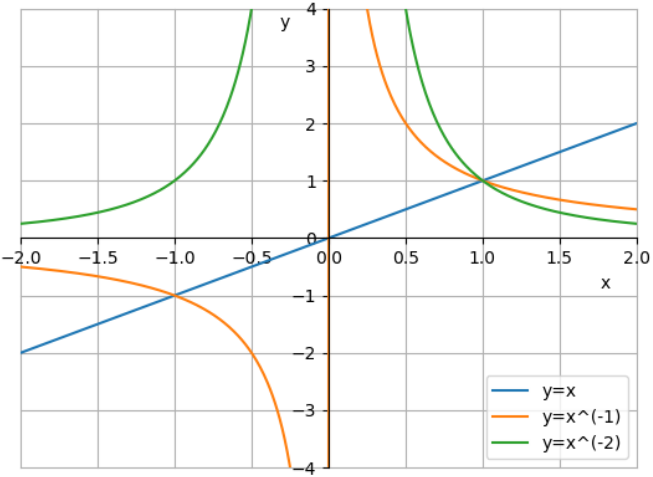
\includegraphics[width=.9\linewidth]{gfx/3/potenze.png}}
\caption{Grafici di funzioni di potenze.}\label{fig:potenze}
\end{figure}

\section{Esponenziale}
Fissata la base $a>0$ con $a \neq 1$, la funzione esponenziale è
\[f(x)=a^x \qquad \dom f = \R \qquad \im f = (0,+\infty)\]
Se si sceglie come base il numero di Nepero $e=2.71828\dots > 1$, la funzione esponenziale si denota:
\[f(x)=e^x=\exp x\]

\subsection{Proprietà}
\begin{enumerate}
	\item se $a>1$, allora la funzzione $a^x$ è strettamente crescente
	\item se $0<a<1$, allora la funzione $a^x$ è strettamente decrescente
	\item se $0<a<b$ con $a,b \neq 1$
	\[\begin{cases}
		a^x<b^x \qquad x>0 \\
		a^x > b^x \qquad x<0
	\end{cases}\]
	\item valgono le seguenti proprietà:
	\begin{itemize}
	\item $a^0=1$
	\item $a^1=a$
	\item $a^{x_1+x_2}=a^{x_1+x_2} \qquad x_1,x_2 \in \R$
	\item $a^{-x}=(\frac{1}{a})^x \qquad x \in \R$
	\item $(a^x)^b = a^{bx} \qquad x,b \in \R$
	\end{itemize}
\end{enumerate}

\begin{figure}[H]
{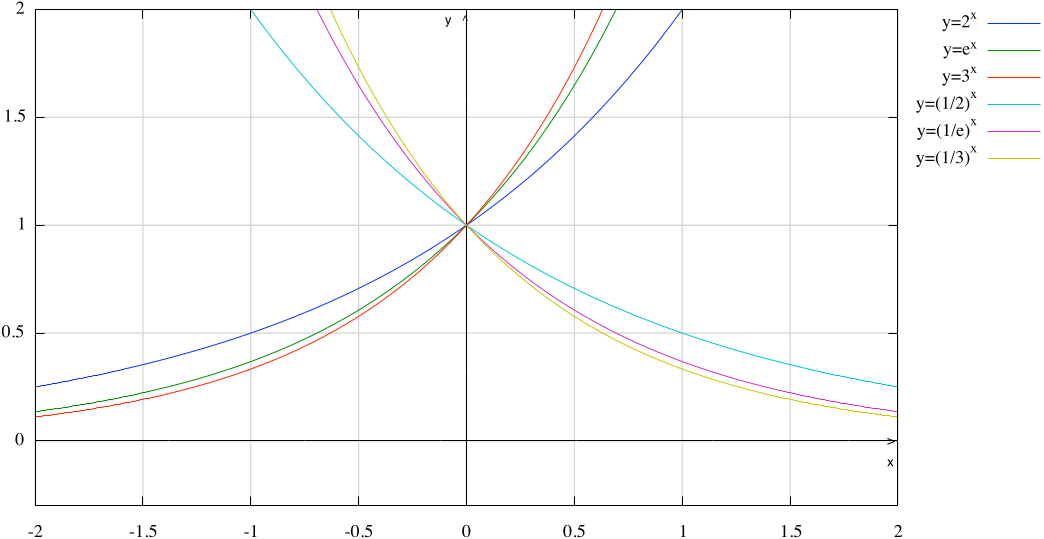
\includegraphics[width=.9\linewidth]{gfx/3/esponenziali.png}}
\caption{Grafici di funzioni esponenziali.}\label{fig:esponenziali}
\end{figure}

\section{Logaritmo}
Fissata la base $a>0$ con $a\neq 1$, la funzione logaritmo
\[f(x)=\log_a x \qquad \dom f = (0,+\infty) \qquad \im f = \R\]
è definita come la funzione inversa della funzione esponenziale $a^x$. Se si sceglie come base il numero di Nepero \textit{e}, il logaritmo si denota:
\[f(x)=\log_e = \log x = \ln x\]

\begin{enumerate}
	\item se $a>1$, allora la funzione $\log_a x$ è strettamente crescente
	\item se $0<a<1$, allora la funzione $\log_a x$ è strettamente decrescente
	\item se $0<a<b$ con $a,b\neq 1$
	\[\begin{cases}
	\log_a x > \log_b x \qquad se x>1 \\
	\log_a x < \log_b x \qquad se 0<x<1 \\
	\end{cases}\]
	\item valgono le seguenti proprietà:
	\begin{itemize}
		\item $\log_a a^x = x \qquad x>1$
		\item $a^{\log_a x}=x \qquad x>0$
		\item $\log_a 1 = 0$
		\item $\log_a a = 1$
		\item $\log_a (x_1 x_2)= \log_a x_1 + \log_a x_2 \qquad x_1,x_2 > 0$
		\item $\log_a (\frac{x_1}{x_2})=\log_a x_1 - \log_a x_2 \qquad x_1,x_2 > 0$
		\item $\log_a x^b = b \log_a x \qquad x>0, b \in \R$
		\item $\log_a x= \frac{\log_b x}{\log_b a}=\frac{\ln x}{\ln a}\qquad x>0,b>0,b\neq 1$
		\item $a^x = e^{(\ln a)x} \qquad x\in \R, a>0, a \neq 1$
	\end{itemize}
\end{enumerate}

\begin{figure}[H]
{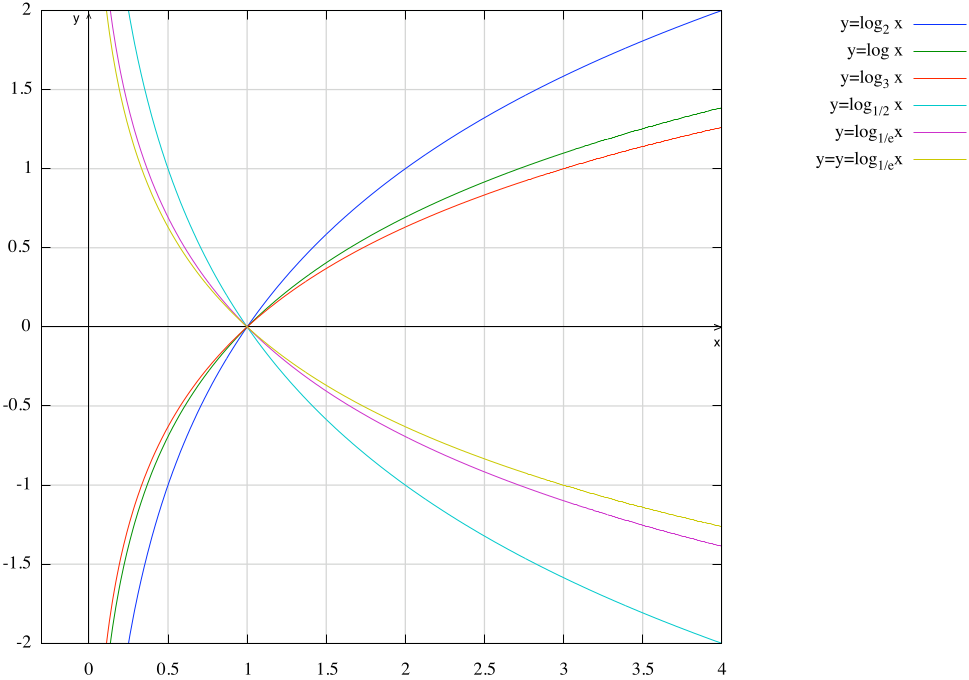
\includegraphics[width=.9\linewidth]{gfx/3/logaritmi.png}}
\caption{Grafici di funzioni logaritmiche.}\label{fig:logaritmi}
\end{figure} % Chapter 3
%% Chapter X

\chapter{Funzioni trigonometriche} % Chapter title

\label{ch:trigonometria} % For referencing the chapter elsewhere, use \autoref{ch:name}

\section{Radianti}

Sia $\gamma$ una circonferenza di raggio $1$ (detta circonferenza goniometrica) il cui centro $O$ è anche l'origine di un sistema di assi cartesiani e sia $A$ il punto $(1,0)$.
Partendo da $A$ percorriamo la circonferenza in senso antiorario oppure in senso orario.
Sia $x$ un numero reale, denotiamo con $P_x$ il punto su $\gamma$ che si ottiene percorrendo la circonferenza a partire dal punto $A$ per un arco di lunghezza $|x|$, in senso antorario se $x \geq 0$, oppure in senso orario se $x<0$.
Il punto $P_x$ individua un angolo nel piano avente vertice $O$ e delimitatio dalle semirette nel piano uscenti da $O$ e passanti per $A$ e per $P_x$.
Il numero reale $x$ rappresenta la misura dell'angolo in radianti.

\begin{wrapfigure}{r}{0.45\textwidth}
  \begin{center}
    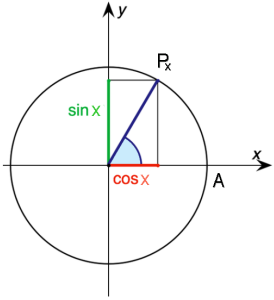
\includegraphics[width=0.42\textwidth]{gfx/4/circonferenza.png}
  \end{center}
  \caption{Circonferenza goniometrica}\label{fig:goniometrica}
\end{wrapfigure}

La relazione tra radianti e gradi è data da:
\[\frac{\gamma_{\text{radianti}}}{2\pi}=\frac{\gamma_{\text{gradi}}}{360}\]

Osserviamo che l'incremento della lunghezza $x$ di $2\pi$ corrisponde a compiere un intero giro sulla circonferenza in senso antiorario ritornando al punto $P_x$ (così come decrementare di $2\pi$ la lunghezza $x$). Quindi si ha:
\[P_{x\pm k2\pi}=P_x \qquad \forall x \in \R, k \in \N\]

\section{Le funzioni seno e coseno}
Una funzione $f:\R \in \R$ è detta periodica di periodo $T$, $T>0$ se:
\[f(x+T)=f(x) \forall x \in \R\]
La caratteristica fondamentale delle funzioni periodiche è che i suoi valori si ripetono dopo intervalli di ampiezza $T$.

\subsection{Simmetria}
Indichiamo con $\cos x$ e con $\sin x$ rispettivamente l'ascissa e l'ordinata del punto $P_x$. Le funzioni $y=\cos x$ e $y=\sin x$ sono definite su $\R$ a valori nell'intervallo $[-1,1]$, sono periodiche di minimo periodo $2\pi$ e soddisfano la relazione:
\[\sin^2 x + \cos^2 x = 1\]

\subsection{Monotonia} Per la periodicità di seno e coseno ci basta studiarne le proprietà nell'intervallo $[0,2\pi]$. Dalle definizioni segue subito che la funzione seno è dispari e la funzione coseno è pari; inoltre la funzione coseno è strettamente decrescente in $[0,\pi]$ e strettamente crescente in $[\pi,2\pi]$. La funzione seno è strettamente crescente in $[0,\frac{\pi}{2}] \cup [\frac{3}{2}\pi,2\pi)$ e strettamente decrescente in $[\frac{\pi}{2},\frac{3}{2}\pi]$.

\begin{figure}[H]
{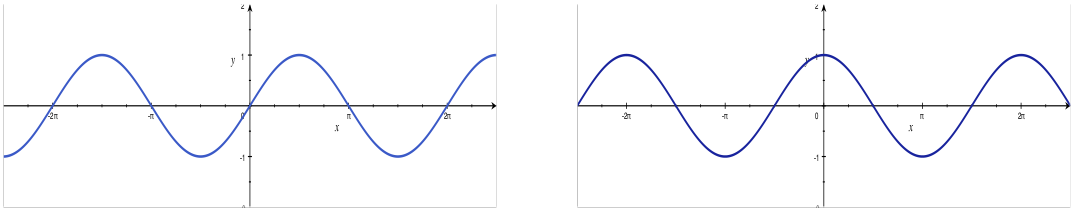
\includegraphics[width=1\linewidth]{gfx/4/senocoseno.png}}
\caption{Grafico delle funzioni: seno e coseno}\label{fig:seno-coseno}
\end{figure}

\subsection{Formule trigonometriche}
\subsubsection{Formule di addizione e sottrazione}
\[\sin(\alpha\pm\beta)=\sin(\alpha)\cos(\beta)\pm\cos(\alpha)\sin(\beta)\]
\[\cos(\alpha\pm\beta)=\cos(\alpha)\cos(\beta)\mp\sin(\alpha)\sin(\beta)\]
\subsubsection{Formule di duplicazione}
\[\sin(2x)=2\sin x\cos x\]
\[\cos(2x)=2\cos^2 x - 1\]
\subsubsection{Formule di potenza}
\[(\sin x)^2 = \sin^2 x= \frac{1-\cos(2x)}{2}\]
\[(\cos x)^2 = \cos^2 x= \frac{1+\cos(2x)}{2}\]
\subsubsection{Formule di bisezione}
\[\sin(\frac{x}{2})=\sqrt{\frac{1-\cos x}{2}} \qquad 0<x\leq 2\pi\]
\[\cos(\frac{x}{2})=\sqrt{\frac{1+\cos x}{2}} \qquad -\pi<x\leq \pi\]
\subsubsection{Formule di prostaferesi}
\[\sin x -\sin y=2\sin(\frac{x-y}{2})\cos(\frac{x+y}{2})\]
\[\cos x -\cos y=-2\cos(\frac{x-y}{2})\sin(\frac{x+y}{2})\]


\[\cos(x+\pi)=-\cos x \qquad \sin(x+\pi)=-\sin x\]
\[\cos(x+\frac{\pi}{2})=-\sin x \qquad \sin(x+\frac{\pi}{2})=\cos x \]

\section{La funzione tangente}
\begin{wrapfigure}{r}{0.45\textwidth}
  \begin{center}
    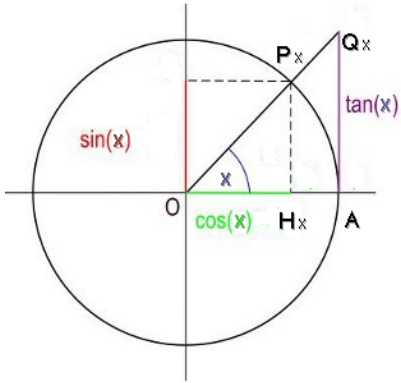
\includegraphics[width=0.42\textwidth]{gfx/4/tangente.png}
  \end{center}
  \caption{Tangente.}\label{fig:circo-tangente}
\end{wrapfigure}

La funzione tangente è:
\[\tan x = \frac{\sin x}{\cos x}\]
Definita nei punti di $\R$ diversi da $\frac{\pi}{2} +k\pi,k\in\Z$ e, come vedremo in seguito, ha immagine $\R$.
La funzione tangente è periodica per: $(x)=\tan(x+k\pi)$ per $k\in \Z$ cioè $\tan(x)$ è periodica di minimo periodo $T=\pi$.

Nella \autoref{fig:circo-tangente} è evidenziata la tangente nel punto $(A,Q_x=\tan(x))$.

\subsection{Simmetria}
Dalle proprietà di simmetria delle funzioni seno e coseno, si deduce che la funzione tangente è dispari: il rapporto di una funzione pari e di una funzione dispari è dispari.

\subsection{Monotonia}
La funzione tangente è strettamente crescente in ogni intervallo $(\frac{-\pi}{2}+k\pi,\frac{\pi}{2}+k\pi), k\in \Z$

\begin{figure}[H]
{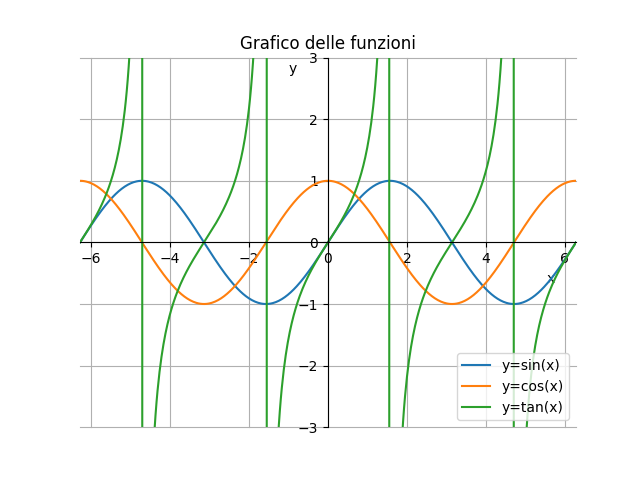
\includegraphics[width=.9\linewidth]{gfx/4/trigonometriche.png}}
\caption{Funzioni trigonometriche}\label{fig:trigonometriche}
\end{figure}

\section{Funzioni trigonometriche inverse}
Le funzioni trigonometriche inverse sono definite come, il dominio della funzione di partenza è stato ristretto per permettere l'inversione della funzione.

\[\arcsin x = f^{-1}(x) \qquad f(x)=\sin(x) \qquad x\in [\frac{-\pi}{2}, \frac{\pi}{2}]\]
\[\arccos x = f^{-1}(x) \qquad f(x)=\cos(x) \qquad x\in [0, \pi]\]
\[\arctan x = f^{-1}(x) \qquad f(x)=\tan(x) \qquad x\in (\frac{-\pi}{2}, \frac{\pi}{2})\]

\subsection{Dominio ed immagine}
\[\dom \arcsin x = [-1,1] \qquad \dom \arccos x = [-1,1] \qquad \dom \arctan x = \R\]
\[\im \arcsin x = [\frac{-\pi}{2}, \frac{\pi}{2}] \qquad \im \arccos x = [0, \pi], \qquad \im \arctan x = (\frac{-\pi}{2}, \frac{\pi}{2})\]

\subsection{Parità}
\[\arcsin(-x)=-\arcsin x\]
\[\arctan(-x)=-\arctan x\]

\subsection{Monotonia}
\begin{itemize}
\item la funzione $\arcsin x$ è strettamente crescente
\item la funzione $\arccos x$ è strettamente decrescente
\item la funzione $\arctan x$ è strettamente crescente
\end{itemize}

\subsection{Relazioni}
\[\arcsin x + \arccos x = \frac{\pi}{2}\]
\[\arccos(-x) = \pi - \arccos(x)\]
\[\arctan x + \arctan (\frac{1}{x}) = \begin{cases}
 \frac{\pi}{2} \quad x>0 \\
 \frac{-\pi}{2} \quad x<0
\end{cases}\]

\begin{figure}[H]
{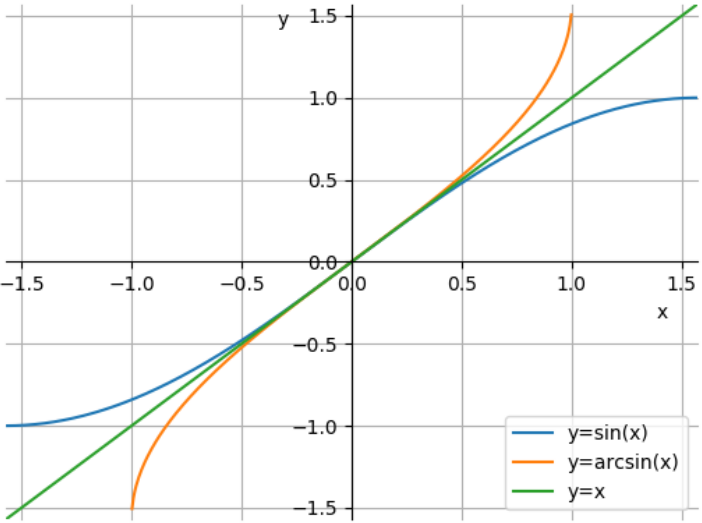
\includegraphics[width=.90\linewidth]{gfx/4/arcoseno.png}}
\caption{Arcoseno.}\label{fig:arcoseno}
\end{figure}

\begin{figure}[H]
{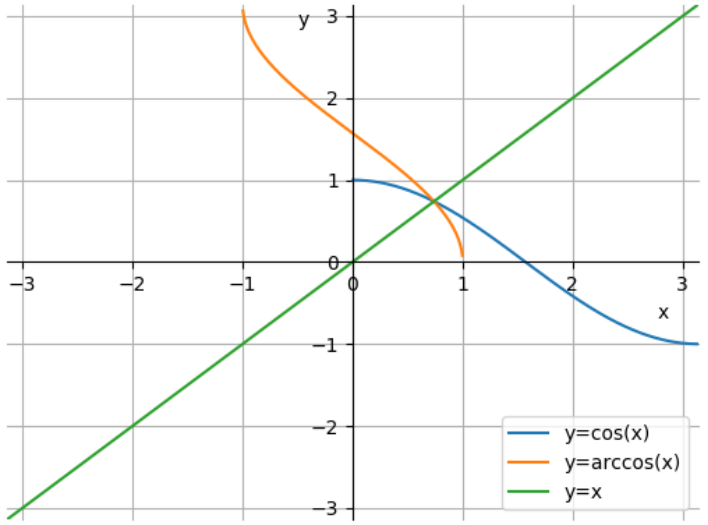
\includegraphics[width=.90\linewidth]{gfx/4/arcocoseno.png}
}
\caption{Arcocoseno.}\label{fig:arcocoseno}
\end{figure}

\begin{figure}[H]
{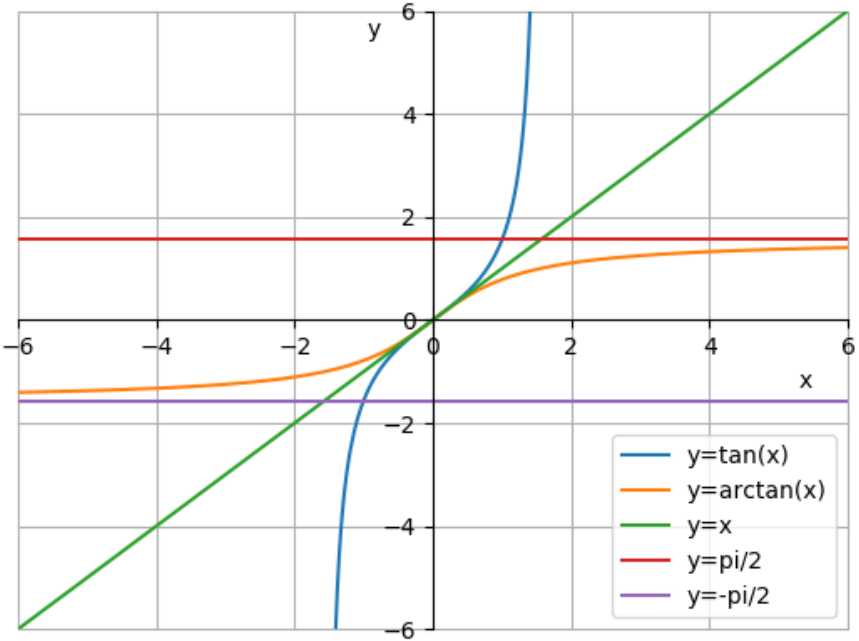
\includegraphics[width=.90\linewidth]{gfx/4/arcotangente.png}}
\caption{Arcotangente.}\label{fig:arcotangente}
\end{figure}
 % Chapter 4 - empty template

\cleardoublepage % Empty page before the start of the next part

%----------------------------------------------------------------------------------------
%	THESIS CONTENT - APPENDICES
%----------------------------------------------------------------------------------------

\appendix

\part{Appendix} % New part of the thesis for the appendix

% Chapter 0a

\chapter{Studio di funzioni} % Chapter title

\label{ch:studio-di-funzioni} % For referencing the chapter elsewhere, use \autoref{ch:name}

%----------------------------------------------------------------------------------------
Lo schema seguente indica i passi principali da seguire per svolgere lo studio di funzioni.

Ogni volta che si è risolto un punto occorre rappresentare l'informazione sul grafico e verificare che sia in accordo con quanto dedotto precedentemente.

\begin{enumerate}
\item Determinare il dominio della funzione $f$ e scriverlo come unione di intervalli:
\[\dom f = I_0 \cup I_1 \cup \dots \]

\item Studiare il segno della funzione e calcolare le intersezioni con gli assi cartesiani: $f(0)$ se $0\in\dom f$ e risolvere l'equazione $f(x)=0$.

\item Stabilire se la funzione è continua, quante vole è derivabile e calcolare $f^\prime$ ed $f^{\prime\prime}$.

\item Calcolare i limiti di $f$ agli estremi di ciascun intervallo, $I_1, I_2 \dots$

\item Studiare il segno della derivata prima $f^\prime$ calcolando i punti critici, deducendo gli intervalli di monotonia della funzione (teorema della caratterizzazione della monotonia).

\item Determinare i punti di massimo e minimo relativi, ricordando che il teorema della condizione necessaria del I ordine dà solo una condizione necessaria affinchè un punto sua un estremo relativo.
\begin{aenumerate}
\item I punti critici $x_0$ (non coincidenti con gli estremi degli intervalli $I_1, I_2 \dots$) in cui la derivata \textit{cambia segno} sono punti di estremo relativo. Infatti, se:
\[\begin{cases}
f^\prime(x)<0 \text{    se } x_0< \delta < x < x_0 \\
f^\prime(x)>0 \text{    se } x_0< \delta < x < x_0 \\
\end{cases}\]
allota $x_0$ è un punto di minimo relativo.
Analogamente se:
\[\begin{cases}
f^\prime(x)>0 \text{    se } x_0< \delta < x < x_0 \\
f^\prime(x)<0 \text{    se } x_0< \delta < x < x_0 \\
\end{cases}\]
allora $x_0$ è un punto di massimo relativo.
Per tali valori, calcolare il corrispondente estremo relativo $f(x_0)$.

\item Verificare se gli estremi degli intervalli $I_1, I_2 \dots$, purchè appartenenti al dominio, siano punti di estremi relativi (in tali punti in generale la derivata prima non si annulla).
Ad esempio se $I_1=[a,b)$ e:
\[f^\prime(x)>0 \qquad a<x<a+\delta\]
allora $x_0=a$ è un punto di minimo relativo, mentre $b\not\in\dom f$ per cui non ha senso chiedersi se sia un punto di estremo relativo.

\item Se lo studio del segno di $f^\prime$ non si può svolgere, ma si riesce a calcolare i punti critici $f^\prime(x_0)=0$, allora il segno di $f^{\prime\prime}(x_0)$ permette di stabilire se è un punto di estremo relativo (Corollario della condizione sufficiente del secondo ordine per estremi relativi).
\end{aenumerate}

\item Determinare $\inf f$ e $\sup f$, stabilendo se sono o meno minimo e massimo assoluti.

\item Determinare l'immagine di $f$ utilizzando il teorema dei valori intermedi.

\item Studiare il segno della derivata seconda $f^{\prime\prime}$ e dedurne gli intervalli di convessità e concavità della funzione (teorema della caratterizzazione convessità).
In particolare i punti in cui $f^{\prime\prime}$ cambia segno, son odetti punti di flesso e, in tali punti, può essere utile calcolare la derivata e tracciare la retta tangente.
\end{enumerate}

In molti casi non si riescono a svolgere esplicitamente i calcoli per tutti i punti e si dovrà dedurre l'andamento del grafico solo attraverso i punti svolti. % Appendix A
%% Chapter 0b

\chapter{Limiti} % Chapter title

\label{ch:limiti-a} % For referencing the chapter elsewhere, use \autoref{ch:name}

%----------------------------------------------------------------------------------------
\section{Limiti notevoli}
\begin{gather}
\lim_{x\to0}{\frac{\sin x}{x}}=1 \\
\lim_{x\to0}{\frac{1-\cos x}{x^2}}=\frac{1}{2} \\
\lim_{x\to0}{\frac{1-\cos x}{x}}=0 \\
\lim_{x\to0}{\frac{a^x-1}{x}} = \ln a \qquad a>0 \\
\lim_{x\to0}{\frac{\log_a(1+x)}{x}}=\frac{1}{\ln a} \\
\lim_{x\to0}{\frac{(1+x)^\lambda-1}{x}}=\lambda \\
\lim_{x\to0}{\frac{e^x-1}{x}}=1 \\
\lim_{x\to0}{\frac{\ln(1+x)}{x}}=1 \\
\lim_{x\to0}{\frac{\tan x}{x}}=1 \\
\lim_{x\to0}{\frac{\arcsin x}{x}}=1 \\
\lim_{x\to0}{\frac{\arctan x}{x}}=1 \\
\lim_{x\to0}{\frac{x}{\log_\alpha(1+x)}}=\frac{1}{\log_\alpha e} \\
\lim_{x\to0}{(1+\alpha x)^{x^{-1}}}=e^\alpha \\
\lim_{x\to0^+}{\left(1+\frac{1}{x}\right)^x}=1 \\
\lim_{x\to1}{\frac{(\arccos x)^2}{1-x}}=2 \\
\lim_{x\to-1^-}{\left(1+\frac{1}{x}\right)^x}=+\infty \\
\lim_{x\to-1^+}{(1+x)^{x^{-1}}}=+\infty \\
\end{gather}

\begin{gather}
\lim_{x\to\infty}{\left(1+\frac{1}{x}\right)^x}=e \\
\lim_{x\to\infty}{\log_\alpha \left(1+\frac{1}{x}\right)^x}=\log_\alpha e \\
\lim_{x\to\infty}{\ln\left(1+\frac{1}{x}\right)^x}=\ln e=1 \\
\lim_{x\to\infty}{\log_a x}=+\infty \\
\lim_{x\to-\infty}{a^x}=0 \\
\lim_{x\to+\infty}{(1+x)^{x^{-1}}}=1 \\
\lim_{x\to\pm\infty}{\left(1+\frac{a}{x}\right)^{bx}}=e^{ab} \\
\end{gather}

\section{Forme indeterminate}
\begin{gather*}
\frac{0}{0} \\
\frac{\infty}{\infty} \\
0\infty \\
1^\infty \\
0^0 \\
\infty^0 \\
+\infty-\infty
\end{gather*} % Appendix B - empty template

%----------------------------------------------------------------------------------------
%	POST-CONTENT THESIS PAGES
%----------------------------------------------------------------------------------------

%\cleardoublepage% Bibliography

\label{app:bibliography} % Reference the bibliography elsewhere with \autoref{app:bibliography}

\manualmark % Work-around to have small caps also here in the headline
\markboth{\spacedlowsmallcaps{\bibname}}{\spacedlowsmallcaps{\bibname}} % Work-around to have small caps also
%\phantomsection
\refstepcounter{dummy}

\addtocontents{toc}{\protect\vspace{\beforebibskip}} % Place the bibliography slightly below the rest of the document content in the table of contents
\addcontentsline{toc}{chapter}{\tocEntry{\bibname}}

\printbibliography % Bibliography

\cleardoublepage% Declaration

\refstepcounter{dummy}
\pdfbookmark[0]{Declaration}{declaration} % Bookmark name visible in a PDF viewer

\chapter*{Declaration} % Declaration section text

\thispagestyle{empty}

Put your declaration here.
\bigskip
 
\noindent\textit{\myLocation, \myTime}

\smallskip

\begin{flushright}
\begin{tabular}{m{5cm}}
\\ \hline
\centering\myName \\
\end{tabular}
\end{flushright}
 % Declaration

\cleardoublepage\pagestyle{empty}

\hfill

\vfill


\pdfbookmark[0]{Colophon}{colophon}
\section*{Colophon}
This document was typeset using the typographical look-and-feel \texttt{classicthesis} developed by Andr\'e Miede and Ivo Pletikosić.
The style was inspired by Robert Bringhurst's seminal book on typography ``\emph{The Elements of Typographic Style}''.
\texttt{classicthesis} is available for both \LaTeX\ and \mLyX:
\begin{center}
\url{https://bitbucket.org/amiede/classicthesis/}
\end{center}
Happy users of \texttt{classicthesis} usually send a real postcard to the author, a collection of postcards received so far is featured here:
\begin{center}
\url{http://postcards.miede.de/}
\end{center}
Thank you very much for your feedback and contribution.

\bigskip

\noindent\finalVersionString

%Hermann Zapf's \emph{Palatino} and \emph{Euler} type faces (Type~1 PostScript fonts \emph{URW
%Palladio L} and \emph{FPL}) are used. The ``typewriter'' text is typeset in \emph{Bera Mono},
%originally developed by Bitstream, Inc. as ``Bitstream Vera''. (Type~1 PostScript fonts were made
%available by Malte Rosenau and
%Ulrich Dirr.)

%\paragraph{note:} The custom size of the textblock was calculated
%using the directions given by Mr. Bringhurst (pages 26--29 and
%175/176). 10~pt Palatino needs  133.21~pt for the string
%``abcdefghijklmnopqrstuvwxyz''. This yields a good line length between
%24--26~pc (288--312~pt). Using a ``\emph{double square textblock}''
%with a 1:2 ratio this results in a textblock of 312:624~pt (which
%includes the headline in this design). A good alternative would be the
%``\emph{golden section textblock}'' with a ratio of 1:1.62, here
%312:505.44~pt. For comparison, \texttt{DIV9} of the \texttt{typearea}
%package results in a line length of 389~pt (32.4~pc), which is by far
%too long. However, this information will only be of interest for
%hardcore pseudo-typographers like me.%
%
%To make your own calculations, use the following commands and look up
%the corresponding lengths in the book:
%\begin{verbatim}
%    \settowidth{\abcd}{abcdefghijklmnopqrstuvwxyz}
%    \the\abcd\ % prints the value of the length
%\end{verbatim}
%Please see the file \texttt{classicthesis.sty} for some precalculated
%values for Palatino and Minion.
%
%    \settowidth{\abcd}{abcdefghijklmnopqrstuvwxyz}
%    \the\abcd\ % prints the value of the length
 % Colophon

%----------------------------------------------------------------------------------------

\end{document}
